\chapter{Dispersão de Ondas de Superfície}

\section{Fundamentos do Método}

Os métodos para determinar a estrutura sísmica da Terra, em particular os métodos tomográficos, baseiam-se num princípio simples: a determinação das velocidades de propagação das ondas sísmicas e a procura de um modelo que melhor se ajuste às velocidades encontradas. A resolução dos modelos obtidos depende do tipo de onda utilizado e da geometria espacial das estações sismigráficas segundo à fonte do sinal. \cite{aki_space_1957} propôs a utilização do ruído sísmico ambiental para medir a dispersão das ondas Rayleigh e Love nas camadas mais superficiais. Somente \cite{campillo_long-range_2003}  e \cite{shapiro_emergence_2004} mostraram, pela primeira vez, a  presença de ondas superficiais nas correlações cruzadas entre pares de estações.

\cite{campillo_long-range_2003}, \cite{shapiro_emergence_2004} e, principalmente, \cite{wapenaar_retrieving_2004} mostram que pode-se recuperar a resposta elástica da Terra a partir da correlação cruzada entre dois pontos em  um campo de ondas difuso ou aleatório. Essa resposta é aproximada como a Função de Green, como é mostrada na equação \ref{crosscorrelation}. 

\cite{boschi_measuring_2013} define a correlação cruzada ($C_{xy}(t,\omega)$) como: 
\begin{eqnarray}
\label{crosscorrelation}
C_{xy}(t,\omega) = \frac{1}{2\pi}\int_{-T}^{T}u(x,t,\omega)u(y,t+\tau,\omega) d\tau
\end{eqnarray}

onde $u$ são sinais registrados em duas estações nas posições $x$ e $y$, $t$ é o tempo, $\omega$ é a frequência, $\tau$ é o atraso e o parâmetro T define o tamanho da janela que a correlação cruzada será computada.
\\

Por possuir inúmeras vantagens em relação aos métodos de análise tradicionais, o número de artigos analisando a dispersão de ondas de superfície cresceu bastante. \cite{shapiro_emergence_2004} lista as seguintes vantagens: as medidas podem ser realizadas em qualquer direção de propagação e não estão limitadas à geometria fonte-receptor; não dependem da localização da fonte; a zona de sensibilidade destas medições situa-se na região que fica entre as duas estações; pode-se analisar pequenos períodos se existirem estações relativamente próximas umas das outras.

\cite{shapiro_emergence_2004} testaram se as funções de Green podem ser extraídas do ruído sísmico ambiental. Neste teste eles selecionaram um
período relativamente calmo no nível de atividade sísmica mundial, onde não ocorreram sismos com magnitude menor que 7. Com esses registos contínuos da componente vertical das estações ANMO e CCM, vistas na Figura \ref{shapiro}-a). Com isso calcularam a correlação cruzada para diferentes bandas de período, mostrado na Figura \ref{shapiro}-b), e aplicaram a análise tempo/frequência para calcular a velocidade de grupo das ondas de superfície segundo \cite{keilis-borok_seismic_2013}. \cite{shapiro_emergence_2004}  compararam as características de dispersão do sinal emergente com mapas preditos para o mesmo trajeto.  Nesta comparação, verificaram que os resultados obtidos para os dois casos são semelhantes.

\begin{figure}[!ht]
\centering
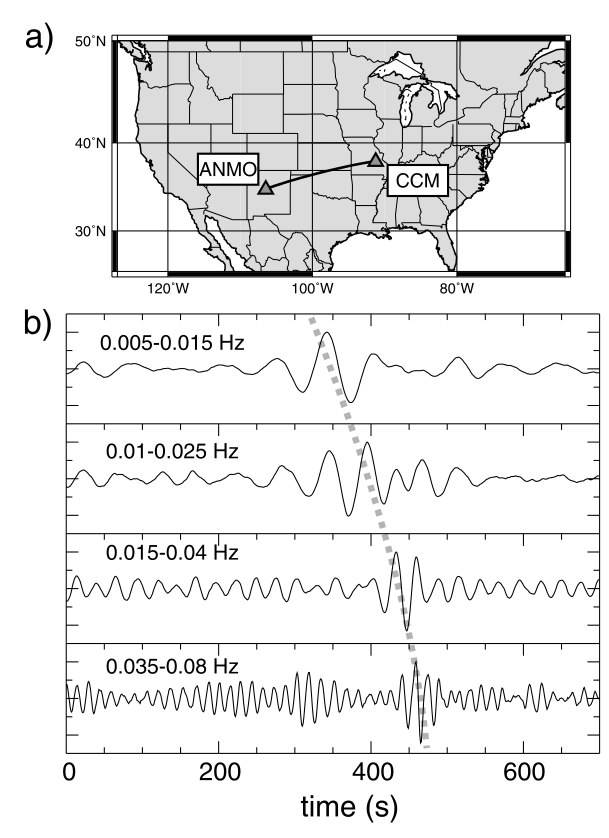
\includegraphics[scale=0.7]{shapiro2004.png}
\caption{(a) Mapa mostrando a localização das estações. (b) Correlações cruzadas da componente vertical dos registros com diferentes filtros de passa-banda, indicados na parte esquerda superior. Linha pontilhada dá 
ênfase na dispersão do sinal emergente. Extraído de \cite{shapiro_emergence_2004}.}
\label{shapiro}
\end{figure} 

\section{Processamento}

Para o processamento dos dados utilizou-se o código escrito pelo Professor Bruno Goutorbe. Tal código engloba a preparação dos dados, o cálculo da correlação, a análise Tempo/frequência e também a inversão tomográfica.  O código está disponível no GitHub no seguinte repositório: https://github.com/bgoutorbe/seismic-noise-tomography.

Todo o fluxo de preparação e processamento dos dados  baseia-se no trabalho de \cite{bensen_processing_2007}. Porém há alterações na filtragem espectral utilizada neste trabalho, devido a utilização de média a baixa frequência no processamento.


\begin{figure}[!ht]
\centering
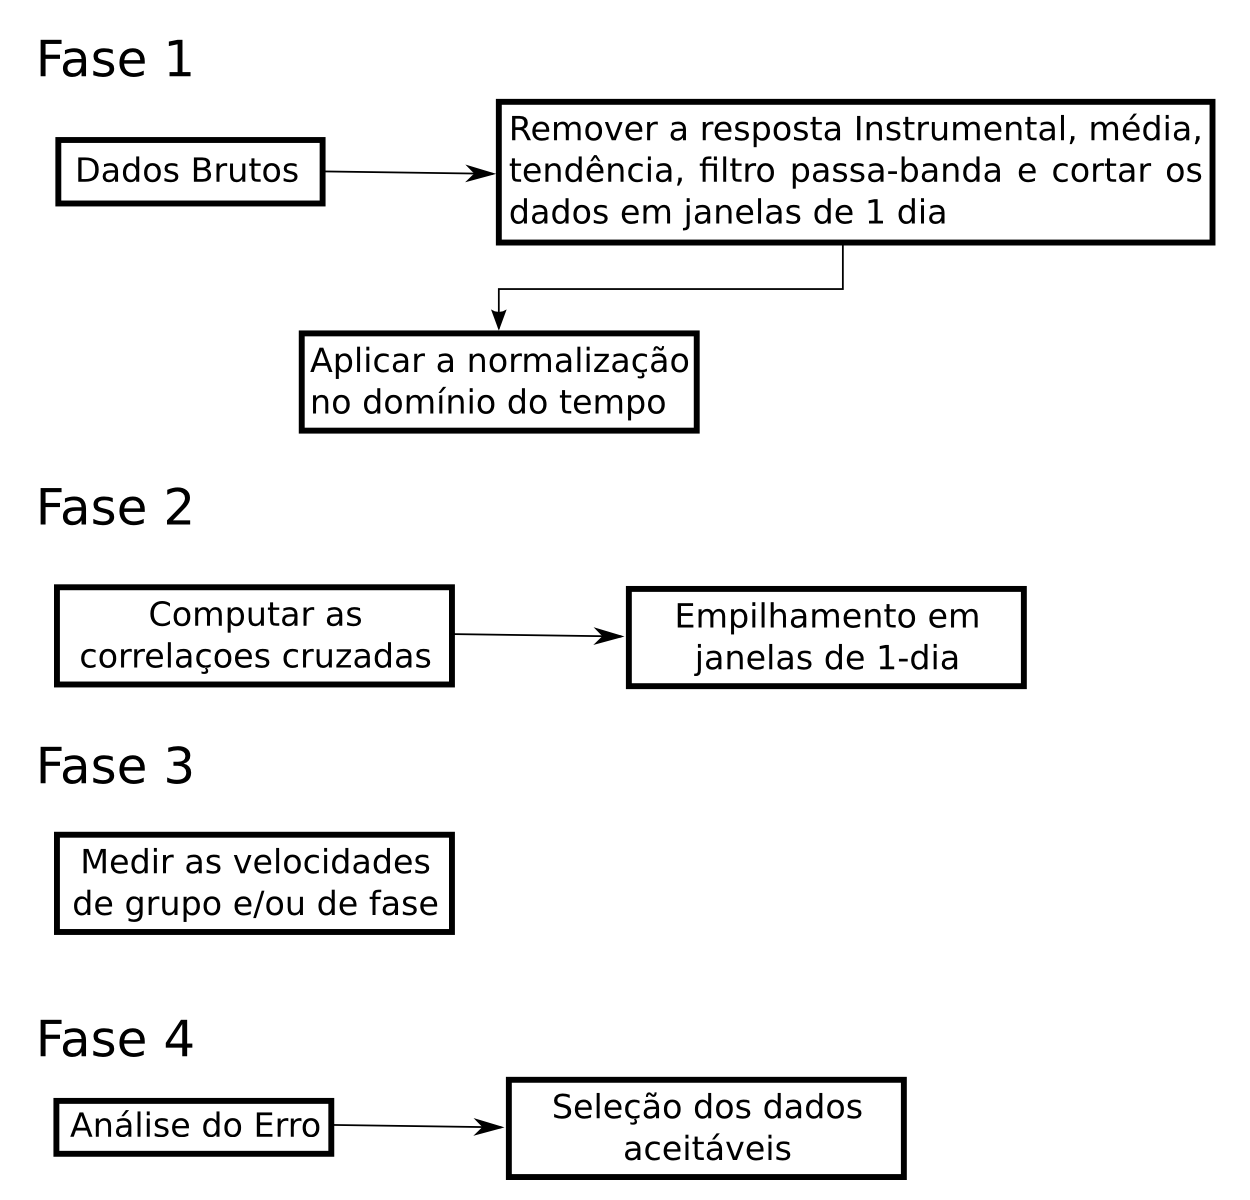
\includegraphics[scale=0.7]{fluxograma_bensen2007.png}
\caption{Representação esquemática do esquema do processamento. Fase 1 mostra as etapas que involvem a preparação dos dados antes da correlação. Fase 2 outlines the cross-correlation procedure and stacking, Phase 3 (Section 4) includes dispersion measurement and Phase 4 (Section 5) is the error analysis and data selection process.. Adaptado de \cite{bensen_processing_2007}.}
\label{fluxograma_bensen2007}
\end{figure} 

\subsection{Preparação dos dados para cada estações}

\cite{bensen_processing_2007} cita que a primeira fase do processamento  é feita para preparar os dados da forma da onda de cada estação individualmente, faz-se isso para acentuar o ruído ambiental de banda larga tentando remover os sinais de terremoto e de irregularidades instrumental que tendem a ocultar o ruído ambiental.

Segundo \cite{bensen_processing_2007}, séries temporáis diárias com menos que 80\% do registro devem ser rejeitadas, mas isso varia de acordo com a discretização do usuário. No caso desse trabalho foram utilizados séries  temporáis diárias com 99\% do registro com o propósito de usar a interpolação o míńimo possível.

Um passo importante na preparação dos dados é a "normalização temporal" ou "normalização no domínio do tempo", \cite{bensen_processing_2007}. Isto é feito para reduzir na correlação cruzada os efeitos de terremotos, irregularidades instrumentais e fontes de ruído não-estacionários próximos á estação. \cite{bensen_processing_2007} compara cinco métodos diferentes para a normalização temporal, como observado na Figura \ref{temporal_norma}.

Terremotos geram grandes impecílios na automatização do processamento, pois eles ocorrem irregularmente e apenas grandes terremotos são encontrados nos catálogos globais, como visto na na Figura \ref{temporal_norma}-a. Então a remoção dos sinais dos terremotos tem que ser adaptativa aos dados. Muitos estudos aplicam a técnica da "normalização 1-bit", como observado na Figura \ref{temporal_norma}-b, em que somente o sinal da série temporal é retido (+1 ou -1) e a amplitude é completamente ignorada. Neste trabalho foi aplicado a "normalização da média absoluta móvel", esta produz uma razão sinal-ruído maior que a normalização 1-bit no conjunto de dados utilizados, estando de acordo com estudos de \cite{seats_improved_2012}.

\begin{figure}[!ht]
\centering
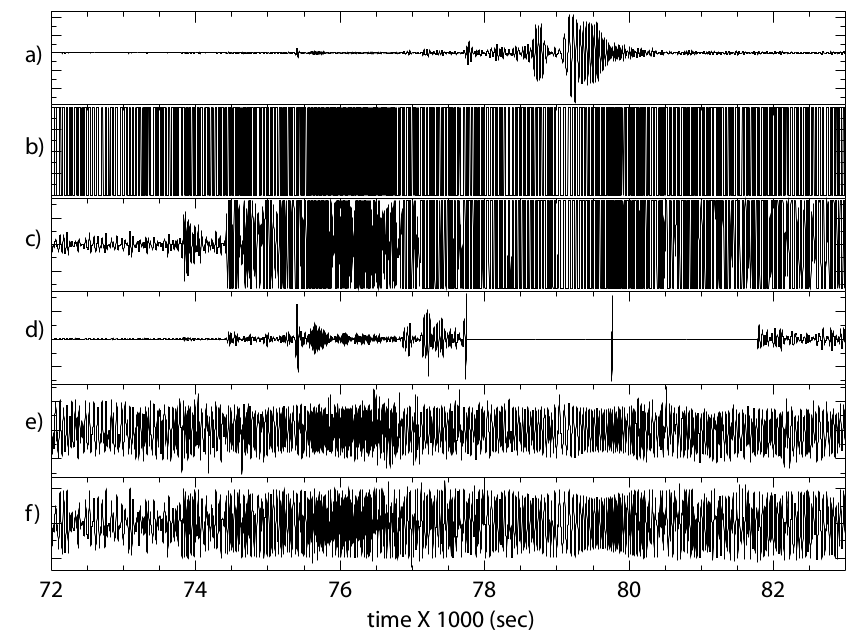
\includegraphics[scale=0.5]{temporal_norma.png}
\caption{Formas de onda mostrando exemplos de cinco tipos de normalização no dominio do tempo testadas por \cite{bensen_processing_2007}. Os exemplos estão com o filtro passa-banda entre 20 e 100 segundos e mostram a contaminação por sinais de terremoto. (a)  Dado bruto mostrando 3 horas de dados janelados em torno de um grande terremoto (M = 7.2, Afeganistão) registrado na estação ANMO. (b) Normalização 1-bit.(c) Forma de onda cortada, onde o limiar de recorte é igual ao rms da amplitude do sinal de um dado dia. (d) Evento detectado e removido automaticamente. (e) Normalização da média absoluta móvel. (f) Normalização ‘\textit{Water level}’ . Retirado de \cite{bensen_processing_2007}.}
\label{temporal_norma}
\end{figure} 

\subsection{Normalização espectral ou braqueamento}

\cite{bensen_processing_2007} cita que a normalização espectral atua para alargar a banda do sinal de ruído ambiental nas correlações cruzadas e também combate a degradação causada por fontes persistentes.

A janela temporal que \cite{bensen_processing_2007} utiliza em seu trabalho é de 7 a 150 segundos, porém quanda a distância entre as estações é pequena ($\simeq 20 km$) é necessário utilizar períodos mais curtos, como é o caso desse trabalho. A janela temporal utilizada é de 2 a 50 segundos, logo há inclusão de ruído de alta frequência.

Com a necessidade de preservar este ruído de baixa frequência não foi aplicada a normalização espectral. 


